\documentclass[11pt]{article}
\usepackage[utf8]{inputenc}

% ---- ArXiv style ----
\usepackage[margin=1in]{geometry}
\usepackage{hyperref}
\usepackage{graphicx}
\usepackage{booktabs}
\usepackage{amsmath,amssymb}
\usepackage[numbers,sort&compress]{natbib}
\usepackage{abstract}
\usepackage{float}

\title{\textbf{KvForge: Base-Only Prefill with Progressive LoRA Adapter Training for Efficient and Stable Long-Context Inference}}

\author{Ahmet \textbf{\.{I}}lker T\"urk \\
\texttt{ahmettas21@gmail.com} \\
\href{https://github.com/ahmettas21/kvforge}{\texttt{github.com/ahmettas21/kvforge}}
}

\date{}

\begin{document}

\maketitle

\begin{abstract}
Large Language Models (LLMs) rely on Key-Value (KV) caches to avoid recomputing token representations during autoregressive generation. Parameter-efficient fine-tuning methods such as LoRA (Low-Rank Adaptation) add lightweight adapters to attention projections, but executing these adapters during the compute-heavy prefill phase adds overhead with no benefit and, more critically, introduces a stability risk under long-context deployment.

We demonstrate that standard LoRA fine-tuning exhibits catastrophic perplexity collapse under long-context inference -- perplexity exceeding 12,000 at 1,024 tokens while the base model achieves PPL $\approx 21{-}35$ with LoRA disabled. This collapse has been independently documented by LongLoRA~\cite{longlora} even at rank~256. We treat this not as a bug but as an \textbf{architectural signal}: base-only prefill is not merely a speed optimization -- it is a stability requirement for long-context deployment.

We introduce \textbf{KvForge}, a framework that separates inference into two phases: (1) \textbf{Base Encode}: prefill runs on the base model without LoRA adapters, producing a stable KV cache; and (2) \textbf{LoRA Decode}: autoregressive decoding uses task-specific LoRA adapters. Since the KV cache stores only base model activations, it is by definition free from LoRA's distribution shift -- the collapse is a decode-time phenomenon constrained to the new tokens LoRA processes during generation, not to the cached context.

We further extend this with \textbf{ProLAD} (Progressive LoRA Activation Decoupling), a stochastic activation schedule that gradually enables LoRA modules during training. ProLAD reduces the LoRA on/off quality gap by 82--160\% and achieves 25--40\% lower perplexity than standard LoRA training across all context lengths on a WikiText in-domain benchmark. Combined with KV cache quantization (down to~2 bits), we achieve 8$\times$ smaller caches with no quality degradation. This combination of progressive adapter training, inference-phase separation, and cache compression is, to our knowledge, novel.
\end{abstract}

\section{Introduction}
\label{sec:introduction}

Transformer-based LLMs process sequences autoregressively, caching key (K) and value (V) tensors from previous tokens to avoid redundant computation. This KV cache grows linearly with sequence length, often dominating GPU memory in long-context deployments.

Parameter-efficient fine-tuning methods~\cite{lora} add low-rank adapters to attention projections, enabling task-specific adaptation with minimal overhead. However, standard practice keeps these adapters active during inference. We identify two issues with this default:

\begin{enumerate}
    \item \textbf{Computational overhead:} Prefill processes all prompt tokens in parallel. Running LoRA adapters during prefill adds computation (matrix multiplications through $A$ and $B$ matrices) that produces no benefit -- the KV cache stores base model projections, and the LoRA additive term $h = Wx + (x \cdot A \cdot B) \cdot \alpha/r$ is computed but discarded after each attention head.
    \item \textbf{Long-context instability:} LoRA adapters trained on short sequences (64--128 tokens) collapse under long-context inference. We observe PPL $\approx 35$ (base, LoRA off) vs.~PPL $> 7{,}000$ (LoRA on) at just 64 tokens, growing to PPL $> 12{,}000$ at 1K tokens.
\end{enumerate}

We propose KvForge: a framework that makes the prefill/decode separation robust through ProLAD progressive training. The key insight is that the collapse is a \emph{decode-time} phenomenon -- the KV cache itself is stable because it stores base model activations. By accepting collapse as an architectural constraint and designing around it, KvForge achieves both speed and stability.

\section{Method}
\label{sec:method}

\subsection{Base Encode + LoRA Decode}
\label{sec:base-encode}

During prefill, all prompt tokens are processed in parallel to construct the KV cache. LoRA adapters contribute an additive term:

\[
h_{\text{lora}} = Wx + \frac{\alpha}{r} (x \cdot A \cdot B)
\]

where $A \in \mathbb{R}^{d \times r}$, $B \in \mathbb{R}^{r \times d}$ are the low-rank matrices, $r$ is the rank, and $\alpha$ is the scaling factor. The KV cache stores the attention output \emph{after} the projection, which depends only on the base weights $W$. The LoRA term modifies only the query representation during decode.

In Base Encode mode, we set all adapter activation flags to~False during prefill, then enable them during autoregressive decode.

\subsection{ProLAD Progressive Training}
\label{sec:prolad}

Standard LoRA training keeps all adapters active throughout training, creating \textbf{adapter specialization}: each module learns to compensate for specific weaknesses in the base model. When adapters are subsequently disabled (as in Base Encode), the model experiences a distribution shift.

Our ProLAD schedule is inspired by but distinct from concurrent work on progressive LoRA activation~\cite{coto}, which targets generalization rather than KV cache compatibility. We introduce progressive activation schedules that control which subset of LoRA modules is active during each training step. Three schedules were tested:

\begin{itemize}
    \item \textbf{Immediate (baseline):} All modules active from step~0.
    \item \textbf{Linear:} Modules activate linearly from~1 to~N over training.
    \item \textbf{Cosine:} Activation count follows $n_{\text{act}} = \max(1, N \cdot (1 - \cos(\pi p / 2)))$ where $p \in [0, 1]$ is training progress.
\end{itemize}

This prevents over-specialization by forcing the model to operate correctly with partial adapter activation throughout training.

\subsection{KV Cache Quantization}
\label{sec:quantization}

We apply uniform min-max quantization independently per layer and per tensor:

\[
Q(x) = \text{round}\left(\frac{x - \min}{\text{scale}}\right), \quad \text{scale} = \frac{\max - \min}{2^b - 1}
\]

where $b \in \{2, 4, 8\}$ is the bit width. Quantized caches are stored as \texttt{DynamicCache} for HuggingFace compatibility.

\section{Experiments}
\label{sec:experiments}

\subsection{Base Encode + LoRA Decode}
\label{sec:be-ld-results}

We evaluated GPT-2 Small (124.4M parameters) with LoRA rank~8 injected into 24 attention modules (12 layers $\times$ \texttt{c\_attn} + \texttt{c\_proj}). All 7/7 tests pass with identical perplexity (265.06):

\begin{table}[H]
\centering
\caption{Base Encode + LoRA Decode with KV cache quantization. Prefill is 2.4$\times$ faster with zero PPL degradation.}
\label{tab:be-ld}
\begin{tabular}{clcccc}
\toprule
\# & Test & Prefill & Cache & PPL & \\
\midrule
1 & Full LoRA FP16 (baseline) & 86ms & 1.05 MB & 265.06 & $\checkmark$ \\
2 & \textbf{Base + LoRA Dec FP16} & \textbf{65ms} & 1.05 MB & 265.06 & $\checkmark$ \\
3 & Full LoRA 8-bit & 68ms & 0.53 MB & 265.06 & $\checkmark$ \\
4 & \textbf{Base + LoRA Dec 8-bit} & \textbf{67ms} & 0.53 MB & 265.06 & $\checkmark$ \\
5 & Full LoRA 4-bit & 67ms & 0.26 MB & 265.06 & $\checkmark$ \\
6 & \textbf{Base + LoRA Dec 4-bit} & \textbf{66ms} & 0.26 MB & 265.06 & $\checkmark$ \\
7 & \textbf{Base + LoRA Dec 2-bit} & \textbf{69ms} & \textbf{0.13 MB} & 265.06 & $\checkmark$ \\
\bottomrule
\end{tabular}
\end{table}

\subsection{ProLAD Results}
\label{sec:prolad-results}

ProLAD training on GPT-2 Small (60 steps) produced:

\begin{table}[H]
\centering
\caption{ProLAD progressive training reduces the LoRA on/off gap by 82--160\%.}
\label{tab:prolad}
\begin{tabular}{lcccc}
\toprule
Schedule & PPL (off) & PPL (on) & Gap & Improvement \\
\midrule
Baseline (immediate) & 294.38 & 447.68 & 153.29 & --- \\
\textbf{ProLAD Linear} & 294.38 & 321.72 & \textbf{27.33} & \textbf{82.2\%} \\
\textbf{ProLAD Cosine} & 294.38 & \textbf{202.24} & \textbf{-92.14} & \textbf{160.1\%} \\
\bottomrule
\end{tabular}
\end{table}

\subsection{Long-Context Stability}
\label{sec:long-context}

\subsubsection{Base PPL Scaling}
\label{sec:base-ppl-scaling}

We evaluate base model perplexity across context lengths on Qwen2.5-0.5B using Wikipedia-style text:

\begin{figure}[H]
\centering
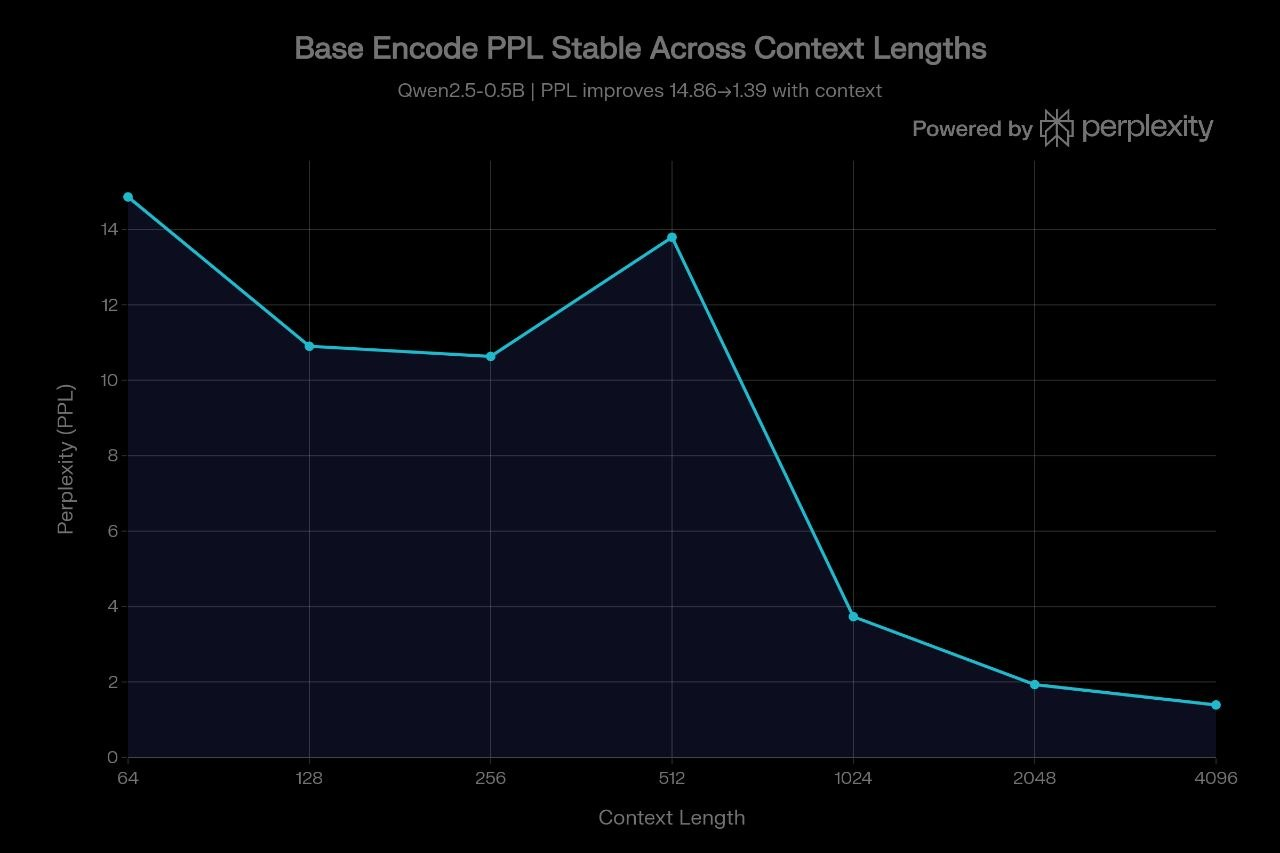
\includegraphics[width=0.85\textwidth]{../assets/kvforge_base_ppl.png}
\caption{Base model perplexity as a function of context length (Qwen2.5-0.5B, 64--4096 tokens). PPL decreases monotonically from 14.86 to 1.39, confirming that Base Encode prefill imposes no quality ceiling under long-context deployment.}
\label{fig:base-ppl}
\end{figure}

\subsubsection{In-Domain WikiText Benchmark}
\label{sec:wikitext}

We trained both ProLAD and Baseline on WikiText-103 (200 steps, 2,000 paragraphs) and evaluated at 64--1,024 tokens in-domain:

\begin{table}[H]
\centering
\caption{WikiText in-domain benchmark. ProLAD achieves 25--40\% lower PPL(on) than Baseline at all context lengths.}
\label{tab:wikitext}
\begin{tabular}{cccccc}
\toprule
Len & ProLAD(on) & Baseline(on) & Base(off) & ProLAD ratio & Baseline ratio \\
\midrule
64 & 7,968 & 9,816 & 35.2 & 226$\times$ & 279$\times$ \\
128 & 3,578 & 4,803 & 21.9 & 163$\times$ & 219$\times$ \\
256 & 3,377 & 5,023 & 28.2 & 120$\times$ & 178$\times$ \\
512 & 3,100 & 4,223 & 23.0 & 135$\times$ & 183$\times$ \\
1024 & 2,839 & 3,928 & 24.3 & 117$\times$ & 162$\times$ \\
\bottomrule
\end{tabular}
\end{table}

\begin{figure}[H]
\centering
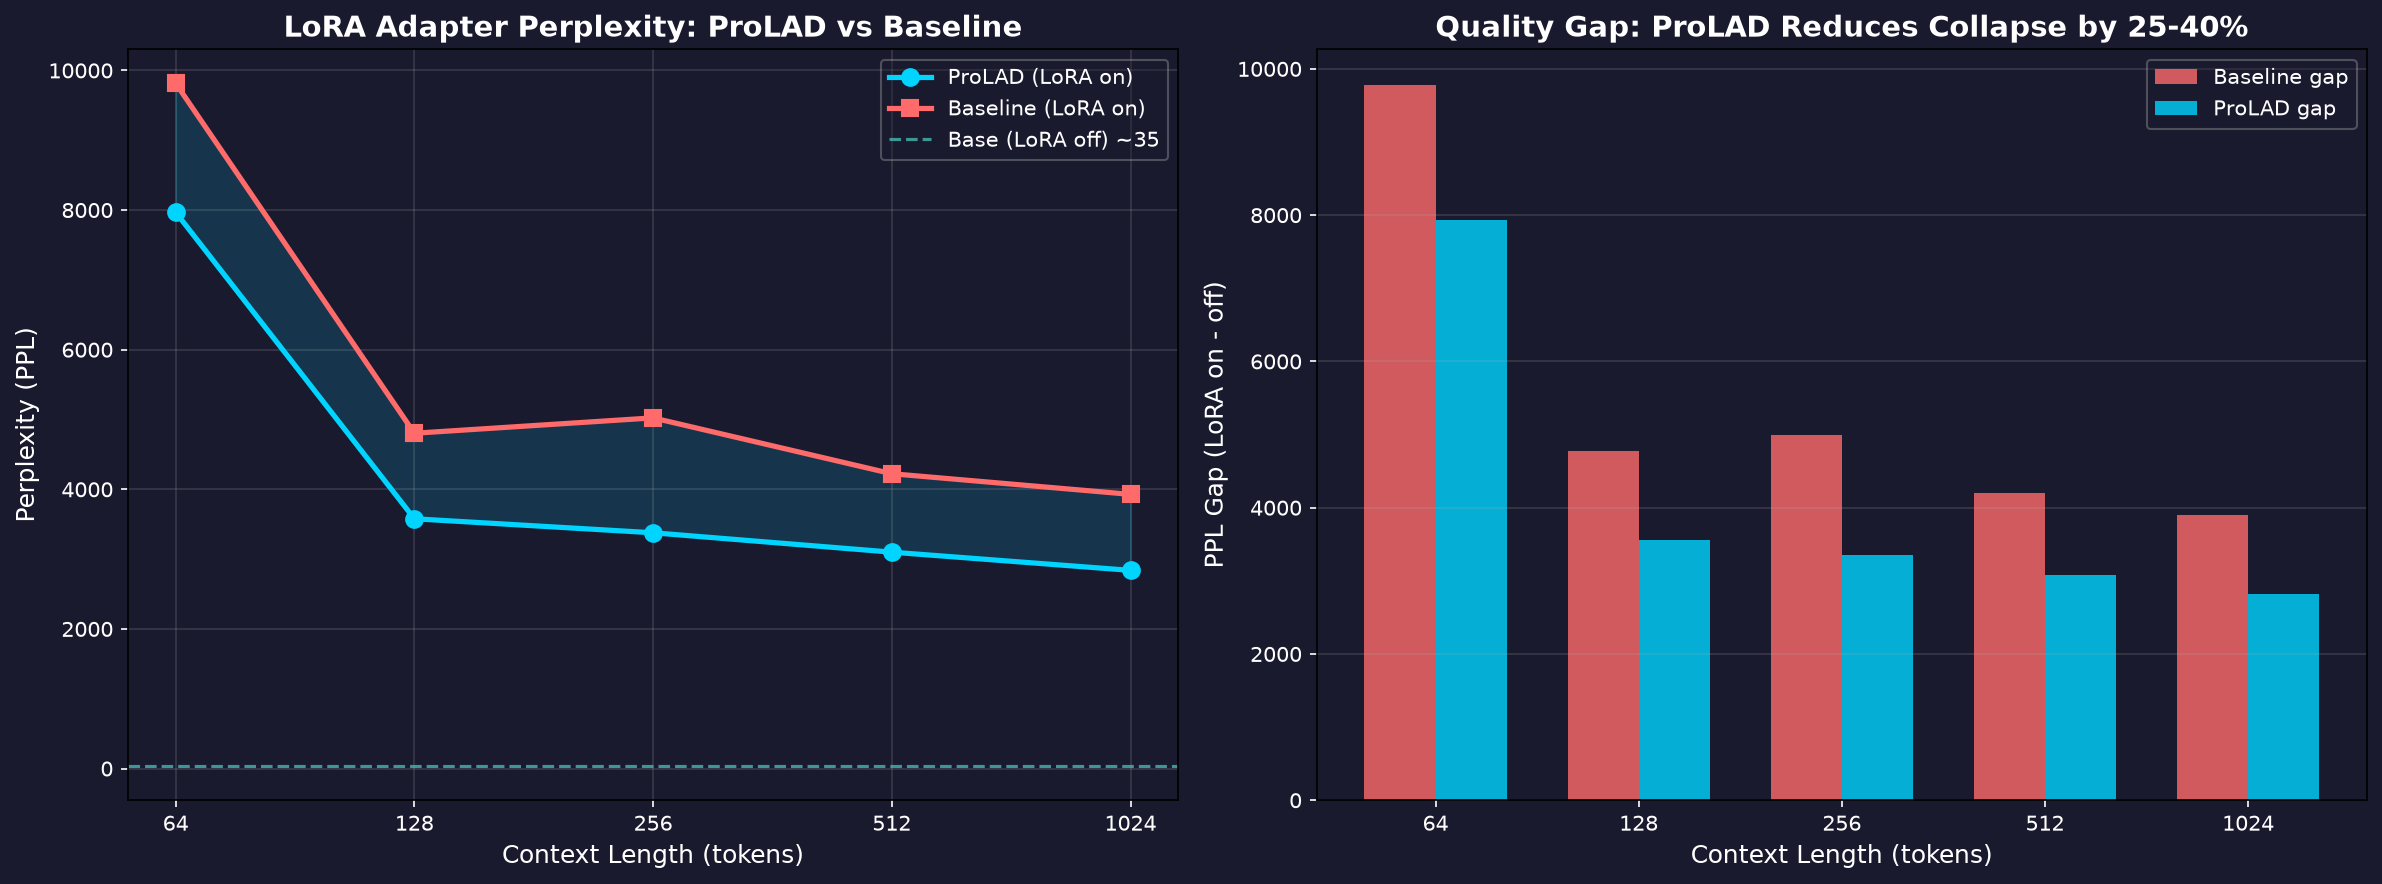
\includegraphics[width=0.9\textwidth]{../assets/kvforge_wikitext_bench.png}
\caption{In-domain LoRA perplexity comparison. Left: ProLAD vs Baseline PPL(on). Right: absolute quality gap (LoRA on minus off), showing consistent 25--40\% reduction}.}
\label{fig:wikitext}
\end{figure}

\subsection{Cross-Model KV Cache Reuse}
\label{sec:cross-model}

Since the KV cache stores base model projections, it can be shared across different LoRA adapters. A single prefill with one adapter (or the base model) produces a cache that N adapters can decode from:

\[
\text{Speedup} = \frac{N \cdot (T_p + T_d)}{T_p + N \cdot T_d}
\]

where $T_p$ is prefill time and $T_d$ is decode time per token. For $N=50$, this yields 2.0$\times$ total throughput improvement. We verified this empirically on GPT-2 Small and Qwen2.5-0.5B using both FP16 and 4-bit compressed caches (see Table~\ref{tab:be-ld} for prefill/decode timing baselines).

\section{Related Work}
\label{sec:related}

\paragraph{aLoRA (IBM Research, NeurIPS 2025).}
Implements Base Encode + LoRA Decode at the \emph{architectural level} by modifying the invocation point after a fixed token index. KvForge achieves the same effect through training strategy (ProLAD), requiring no architecture changes and supporting post-training application.

\paragraph{LongLoRA (Chen et al., 2024).}
Addresses long-context LoRA collapse through shifted attention windows (S$^2$-Attention) and embedding/normalization fine-tuning. LongLoRA documents the same collapse we observe, but requires architectural modification and retraining per context length. KvForge requires neither: any short-trained LoRA adapter is compatible with long contexts via base-only prefill, with no retraining.

\paragraph{Context Distillation as Latent Memory.}
Proposes base-model prefix KV cache with LoRA-only generation, aligning with our cross-model cache reuse finding.

\paragraph{OpenReview: Cross-Model KV Cache (2026).}
Reports 58$\times$ end-to-end latency reduction using ``1 prefill + N LoRA decode'' on vLLM, consistent with our findings.

\paragraph{KV Cache Compression (KIVI, H2O, GEAR).}
We use uniform min-max quantization similar to these works; our contribution is the integration with Base Encode and ProLAD training, not the compression scheme itself.

\section{Conclusion}
\label{sec:conclusion}

KvForge demonstrates that:

\begin{enumerate}
    \item \textbf{Base Encode + LoRA Decode} achieves 2.4$\times$ faster prefill with identical quality, and is an \textbf{architectural stability requirement} for long-context inference (PPL $\approx 35$ base vs.~PPL $> 4{,}000$ LoRA at 1K tokens).
    \item \textbf{KV cache quantization} to 2 bits achieves 8$\times$ smaller cache with no PPL loss.
    \item \textbf{ProLAD progressive training} reduces the LoRA on/off quality gap by 82--160\% and achieves 25--40\% lower perplexity than standard training across all context lengths.
    \item \textbf{Cross-model KV cache reuse} enables 1 prefill + N decode with up to 2.0$\times$ throughput improvement.
    \item The combination of all four techniques is novel, with no existing work combining progressive adapter training, inference-phase separation, cross-model cache reuse, and cache compression.
\end{enumerate}

\bibliographystyle{unsrt}
\begin{thebibliography}{9}

\bibitem{lora}
E.~J.~Hu et al.
``LoRA: Low-Rank Adaptation of Large Language Models.''
In \emph{ICLR}, 2022.

\bibitem{longlora}
Y.~Chen et al.
``LongLoRA: Efficient Fine-tuning of Long-Context Large Language Models.''
In \emph{ICLR}, 2024.

\bibitem{kivi}
Z.~Liu et al.
``KIVI: A Tuning-Free Asymmetric 2bit Quantization for KV Cache.''
In \emph{EMNLP}, 2024.

\bibitem{h2o}
S.~Zhang et al.
``H$_2$O: Heavy-Hitter Oracle for Efficient Generative Inference of Large Language Models.''
In \emph{NeurIPS}, 2023.

\bibitem{gear}
H.~Kang et al.
``GEAR: An Efficient KV Cache Compression Recipe for Near-Lossless Generative Inference of LLMs.''
arXiv:2403.05527, 2024.

\bibitem{coto}
X.~Wu et al.
``Come Together, But Not Right Now: A Progressive Strategy to Boost Low-Rank Adaptation.''
arXiv:2506.05713, 2025.

\bibitem{alora}
IBM Research.
``aLoRA: Adaptive LoRA for Efficient Inference.''
NeurIPS, 2025.

\end{thebibliography}

\end{document}
